% Source for the figure of BoundaryTagAllocator (sec. 5.2): a memory of 24
% words before and after free(7), which merges the freed block with both its
% free neighbors; each block has its tags at its two ends (+s free, -s in
% use), and a free block its links in its second and third words. Build:
% make figures (in ../build).
\documentclass[border=4pt]{standalone}
\usepackage[T1]{fontenc}
\usepackage{newpxtext,newpxmath}
\usepackage[varqu,varl,scaled=0.95]{zi4}
\usepackage{tikz}
% tikz-ads.tex: the TikZ styles shared by the figures of the memory of the
% manual, \input by each standalone figure: a cell of a vector (cell), the
% cell that an operation touches (touched), a free cell (free), a node of a
% linked structure (node), the labels of indices (index) and of variables
% (var), a pointer (ptr), and \cells and \indices to draw a row of cells.
\usetikzlibrary{arrows.meta,positioning,calc,fit,shapes.multipart}
\definecolor{adsTouched}{RGB}{214,196,236}
\definecolor{adsFree}{RGB}{236,236,236}
\tikzset{
  ads/.style={>={Stealth[length=2mm]},font=\small,
              every node/.append style={inner sep=0pt}},
  cell/.style={draw,minimum width=7mm,minimum height=7mm,
               font=\small\ttfamily,outer sep=0pt},
  touched/.style={cell,fill=adsTouched},
  free/.style={cell,fill=adsFree,text=black!45},
  node/.style={draw,rounded corners=1pt,minimum width=8mm,
               minimum height=6mm,font=\small\ttfamily},
  index/.style={font=\scriptsize\ttfamily,text=black!60},
  var/.style={font=\small\itshape},
  ptr/.style={->,thick}
}
% \cells{name}{x,y}{list}: a row of cells, the first at (x,y), named
% name-0, name-1, ...; each item is text/style, the style one of cell,
% touched and free (e.g., {a/cell,e/touched,/free})
\newcommand{\cells}[3]{%
  \foreach \v/\s [count=\i from 0] in {#3}
    \node[\s] (#1-\i) at ($(#2)+(\i*7mm,0)$) {\v};}
% \indices{name}{n}: the indices 0 .. n-1 under the cells of name
\newcommand{\indices}[2]{%
  \foreach \i in {0,...,\numexpr#2-1\relax}
    \node[index,below=1.2mm of #1-\i] {\i};}

% \word{x}{y}{style}{text}: a word of 6 mm at the place x of the row y
\newcommand{\word}[4]{\node[#3,minimum width=6mm,minimum height=6mm,
  font=\scriptsize\ttfamily] at (#1*6mm,#2) {#4};}
% \blk{a}{b}{y}: the outline of the block of the places a .. b of the row y
\newcommand{\blk}[3]{\draw[very thick] (#1*6mm-3mm,#3-3mm) rectangle
  (#2*6mm+3mm,#3+3mm);}
\begin{document}
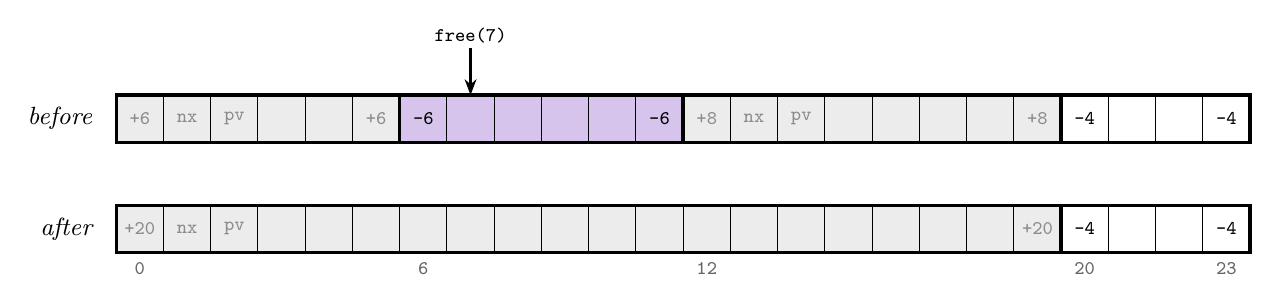
\begin{tikzpicture}[ads]
  % before: free [0,6), in use [6,12), free [12,20), in use [20,24)
  \node[var,anchor=east] at (-6mm,0) {before};
  \foreach \i/\t in {0/+6,1/nx,2/pv,3/,4/,5/+6}{\word{\i}{0}{free}{\t}}
  \foreach \i/\t in {6/-6,7/,8/,9/,10/,11/-6}{\word{\i}{0}{touched}{\t}}
  \foreach \i/\t in {12/+8,13/nx,14/pv,15/,16/,17/,18/,19/+8}{\word{\i}{0}{free}{\t}}
  \foreach \i/\t in {20/-4,21/,22/,23/-4}{\word{\i}{0}{cell}{\t}}
  \blk{0}{5}{0}\blk{6}{11}{0}\blk{12}{19}{0}\blk{20}{23}{0}
  \draw[ptr] (7*6mm,9mm) node[above=0.5mm,font=\scriptsize\ttfamily] {free(7)}
    -- (7*6mm,3mm);
  % after: free [0,20), in use [20,24)
  \node[var,anchor=east] at (-6mm,-14mm) {after};
  \foreach \i/\t in {0/+20,1/nx,2/pv,3/,4/,5/,6/,7/,8/,9/,10/,11/,12/,13/,14/,15/,16/,17/,18/,19/+20}
    {\word{\i}{-14mm}{free}{\t}}
  \foreach \i/\t in {20/-4,21/,22/,23/-4}{\word{\i}{-14mm}{cell}{\t}}
  \blk{0}{19}{-14mm}\blk{20}{23}{-14mm}
  \foreach \i in {0,6,12,20,23}
    \node[index] at (\i*6mm,-19mm) {\i};
\end{tikzpicture}
\end{document}
